\subsection{Optimization}
To train a FFNN, we need to optimize the parameters of the network to minimize the loss function. 
This is usually done using gradient-based optimization algorithms, such as gradient descent and its variants. 

These algorithms are based on the idea of iteratively updating the parameters of the network in the direction of the steepest descent
of the loss function, which is given by the negative of the gradient of the loss function with respect to the parameters.
To better understand this, let's first introduce the concept of gradients.

\subsubsection{Gradients}
Gradients are a vector of partial derivatives that indicate the \textbf{direction} and \textbf{magnitude} of the \textbf{steepest ascent} of a function. 
Given the loss function $\mathcal{L}(\boldsymbol{W})$, the gradient with respect to the parameters $w_i$ is given by:
\begin{equation*}
    \nabla_{w_i} \mathcal{L} = \left[ \frac{\partial \mathcal{L}}{\partial w_1}, \frac{\partial \mathcal{L}}{\partial w_2}, \ldots, \frac{\partial \mathcal{L}}{\partial w_N} \right]
\end{equation*}
Each component of the gradient vector $\frac{\partial \mathcal{L}}{\partial w_i}$ measures the rate of change of the loss function 
with respect to each parameter.
\begin{figure}[H]
    \centering
    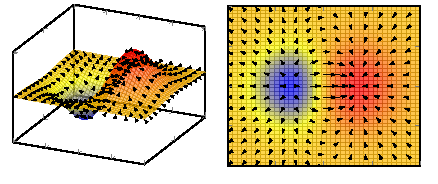
\includegraphics[width=\textwidth]{chapters/02-ffnn/media/partial_derivatives.pdf}
    \caption{Visualization of derivatives and gradients.}
\end{figure}
If we move on the opposite side of the gradients, we will be moving in the direction of the \textbf{steepest descent} of the loss function.
This way, these algorithms can iteratively explore the parameter space to find the optimal parameters that minimize the loss function.
\begin{figure}[H]
    \centering
    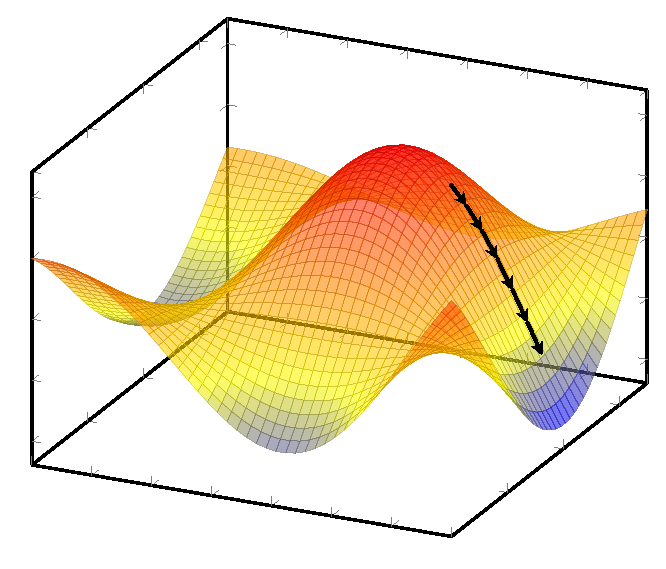
\includegraphics[width=\textwidth]{chapters/02-ffnn/media/gradient-descent.pdf}
    \caption{Visualization of Gradient Descent.}
\end{figure}

\subsubsection{Problems with gradients}
By now we know that in neural networks, the loss function is usually non-convex, which means that it can have multiple local minima and saddle points.

\paragraph{Local minima} Local minima are points in the parameter space where the loss function has a lower value than in the surrounding area,
but it is not the global minimum. This can lead to suboptimal performance of the model.

\paragraph{Saddle points} Similarly, saddle points are points in the parameter space where the loss function has a gradient of zero,
but does not correspond to a local minimum.

Both local minima and saddle points are issues that can arise during the optimization process. Altough they can lead to suboptimal performance,
there are still other issues regarding optimization, that are much more important.
\subsubsection{Gradient Descent}

\subsubsection*{Batch Gradient Descent}
Batch Gradient Descent is an optimization algorithm used to minimize the loss function by iteratively updating the parameters of the model
in the direction of the negative gradient of the loss function with respect to the parameters.

In the general case, we can express the update rule for the parameters $\boldsymbol{\theta}$ as follows:

\begin{algorithm}[H]
    \caption{Batch Gradient Descent}
    \begin{algorithmic}[1]
        \Require{Learning rate $\eta$}
        \Require{Initial parameters $\boldsymbol{\theta}$}
        \While {stopping criteria not met}
            \State Compute \textbf{gradient} estimate over the entire dataset:
            \State $\nabla \leftarrow \frac{1}{N} \sum\limits_{i=1}^{N} \nabla_{\boldsymbol{\theta}} \mathcal{L}(f(\boldsymbol{x}^{(i)}; \boldsymbol{\theta}), y^{(i)})$
            \State $\boldsymbol{\theta} \leftarrow \boldsymbol{\theta} - \eta \nabla$
        \EndWhile
        \State \textbf{Output:} Learned parameters $\boldsymbol{\theta}$
    \end{algorithmic}
\end{algorithm}
where $\eta$ is the learning rate, which controls the step size of the updates and some parameter initialization is required to start the optimization process.

This allows for more stable gradient updates. However, computing the gradient over the entire dataset can be computationally expensive, especially for large datasets.

\begin{definition}{Remarks on Learning Rate}
    {
        For better result, the learning rate $\eta$ should be adjusted during training, starting with a higher 
        value and gradually decreasing it as the optimization process progresses.
        This can be defined trough the Learning Rate Schedule:
        \begin{equation*}
            \eta_k = (1 - \alpha)\eta_0 + \alpha \eta_{\tau}\;\;\alpha = \frac{k}{\tau}
        \end{equation*}
        
        The starting value of the learning must be choosen by trying different values and analyzing the 
        learning curves on the validation set.
        \begin{itemize}
            \item If the Learning Rate is too large, the curves will show big oscillations.
            \item If it is too low, learning proceeds too slowly.
        \end{itemize}
    }
\end{definition}

\subsubsection*{Stochastic Gradient Descent}
Stochastic Gradient Descent (SGD) is a variant of gradient descent that updates the parameters using only a single training example at a time, allowing for faster updates and convergence.
The update rule for SGD can be expressed as follows:
\begin{algorithm}[H]
    \caption{Stochastic Gradient Descent}
    \begin{algorithmic}[1]
        \Require{Learning rate $\eta$}
        \Require{Initial parameters $\boldsymbol{\theta}$}
        \While {stopping criteria not met}
            \State $i \leftarrow$ randomly selected index from $\{1, 2, \ldots, N\}$
            \State $\nabla \leftarrow \nabla_{\boldsymbol{\theta}} \mathcal{L}(f(\boldsymbol{x}^{(i)}; \boldsymbol{\theta}), y^{(i)})$
            \State $\boldsymbol{\theta} \leftarrow \boldsymbol{\theta} - \eta \nabla$
        \EndWhile
        \State \textbf{Output:} Learned parameters $\boldsymbol{\theta}$
    \end{algorithmic}
\end{algorithm}
This allows for faster updates and convergence, but causes a non-smooth optimization process.
This is not always a bad thing, as it can help to escape local minima and saddle points, but it can also lead to more noisy updates and slower convergence.

\subsubsection*{Mini Batch}
To mitigate the issues of both Batch Gradient Descent and Stochastic Gradient Descent, we can use Mini Batch Gradient Descent. Instead
of using the entire dataset or a single training example, we can use a small batch of training examples to compute the gradient and update the parameters.
The size of the mini batch is a hyperparameter that can be tuned based on the specific problem, dataset size, and hardware constraints.

This has many advantages. First, its computation isn't dependent on the size of the dataset anymore,
allowing computations on extremly large datasets.
Secondly, it allows for parallelization of the computations, as we can compute the gradients for each mini batch in parallel, which can significantly speed up the training process.
Finally, it provides a good balance between the stability of Batch Gradient Descent and the speed of Stochastic Gradient Descent.

However, along flat direction of the loss function, the gradient steps can be very small, leading to slow convergence.
In steep ravines, the gradient steps can be very large, leading to oscillations and divergence.
To mitigate these issues, the concept of momentum was introduced.

\subsubsection{SGD with Momentum}
To solve the issues of slow convergence along flat directions and oscillations in steep ravines, we can introduce the concept of momentum into the SGD algorithm.

The idea is to introduce a \textbf{velocity} term $v$ that accumulates the gradients over time, allowing for faster convergence and smoother updates.
This can be represented by exponentially decaing moving average of the negative gradients, which can be expressed as follows:
\begin{equation*}
    v \leftarrow \alpha v - \eta \nabla_{\boldsymbol{\theta}} (\mathcal{L}(f(\boldsymbol{x}^{(i)}; \boldsymbol{\theta}), y^{(i)}))
\end{equation*}
Where $\alpha$ is the momentum hyperparameter that controls the contribution of the previous velocity to the current update.

The update rule for the parameters can then be expressed as follows:
\begin{algorithm}[H]
    \caption{Stochastic Gradient Descent with Momentum}
    \begin{algorithmic}[1]
        \Require{Learning rate $\eta$}
        \Require{Momentum hyperparameter $\alpha$}
        \Require{Initial velocity $v$}
        \Require{Initial parameters $\boldsymbol{\theta}$}
        \While {stopping criteria not met}
            \State $i \leftarrow$ randomly selected index from $\{1, 2, \ldots, N\}$
            \State $\nabla \leftarrow \nabla_{\boldsymbol{\theta}} \mathcal{L}(f(\boldsymbol{x}^{(i)}; \boldsymbol{\theta}), y^{(i)})$
            \State $v \leftarrow \alpha v - \eta \nabla$
            \State $\boldsymbol{\theta} \leftarrow \boldsymbol{\theta} + v$
        \EndWhile
        \State \textbf{Output:} Learned parameters $\boldsymbol{\theta}$
    \end{algorithmic}
\end{algorithm}

\begin{figure}[H]
    \centering
    \scalebox{0.3}{\definecolor{ovalcolor}{RGB}{180,180,180}
\colorlet{myred}{red!80!black}
\colorlet{myblue}{blue!80!black}
\colorlet{mybluee}{myblue!80!black}
\colorlet{mygreen}{green!60!black}
\colorlet{mydarkred}{red!30!black}
\colorlet{mydarkblue}{blue!40!black}
\colorlet{mydarkgreen}{green!30!black}

\begin{tikzpicture}[>=Stealth, scale=0.75]

% ===== Contours =====
\foreach \shift in {-6, 12, 30}{
\begin{scope}[shift={(\shift,0)}]
    \foreach \r in {1,...,6}{
        \draw[ovalcolor, thick, rotate=145] (0,0) ellipse ({\r*1.5} and {\r});
    }
\end{scope}
}

% ===== Labels =====
\node at (-4.5,-8.9) {\huge\textbf{Batch Gradient Descent}};
\node at (13.5,-8.9) {\huge\textbf{Stochastic Gradient Descent}};
\node at (31.5,-8.9) {\huge\textbf{SGD with Momentum}};

% ===== Batch Gradient Descent (straight line) =====
\foreach \i in {0,...,9}{
\draw[line width=3pt, myred, -{Stealth[round,color=mydarkred]}]
(-6.6-0.6*\i,0.6+0.6*\i) -- (-5.8-0.6*\i,-0.2+0.6*\i);
}
% ===== Stochastic Gradient Descent (zig-zag line) =====
\draw [line width=3pt, mybluee, arrows = {-Stealth[round,color=mydarkblue]}] (11.0,0.2) -- (12.0,0);
\draw [line width=3pt, mybluee, arrows = {-Stealth[round,color=mydarkblue]}] (13.6,0.6) -- (10.5,0.2);
\draw [line width=3pt, mybluee, arrows = {-Stealth[round,color=mydarkblue]}] (8.1,0.9) -- (13.7,0.7); 
\draw [line width=3pt, mybluee, arrows = {-Stealth[round,color=mydarkblue]}] (13.8,2.2) -- (8.1,1); 
\draw [line width=3pt, mybluee, arrows = {-Stealth[round,color=mydarkblue]}] (6.2,1.9) -- (13.9,2.3); 
\draw [line width=3pt, mybluee, arrows = {-Stealth[round,color=mydarkblue]}] (13.6,3.6) -- (6.3,2); 
\draw [line width=3pt, mybluee, arrows = {-Stealth[round,color=mydarkblue]}] (7.1,3.4) -- (13.7,3.7);

\draw [line width=3pt, mybluee, arrows = {-Stealth[round,color=mydarkblue]}] (11.4,4.7) -- (6.9,3.3); 
\draw [line width=3pt, mybluee, arrows = {-Stealth[round,color=mydarkblue]}] (6.6,5.1) -- (11.6,4.6);
\draw [line width=3pt, mybluee, arrows = {-Stealth[round,color=mydarkblue]}] (11.4,6.7) -- (6.4,5); 
\draw [line width=3pt, mybluee, arrows = {-Stealth[round,color=mydarkblue]}] (6.3,6.5) -- (11.6,6.7);


% ===== Momentum (COMPLETELY REDONE: shorter, damped path near top) =====
\draw [line width=3pt, mygreen, arrows = {-Stealth[round,color=mydarkgreen]}] (28.4,0.2) -- (30,0);
\draw [line width=3pt, mygreen, arrows = {-Stealth[round,color=mydarkgreen]}] (30.8,0.7) -- (28.5,0.3);
\draw [line width=3pt, mygreen, arrows = {-Stealth[round,color=mydarkgreen]}] (27.1,1.1) -- (30.9,0.8);

\draw [line width=3pt, mygreen, arrows = {-Stealth[round,color=mydarkgreen]}] (30.4,1.9) -- (27.2,1.2);
\draw [line width=3pt, mygreen, arrows = {-Stealth[round,color=mydarkgreen]}] (25.8,2.4) -- (30.5,2);
\draw [line width=3pt, mygreen, arrows = {-Stealth[round,color=mydarkgreen]}] (30.1,3.2) -- (25.9,2.5);
\draw [line width=3pt, mygreen, arrows = {-Stealth[round,color=mydarkgreen]}] (25.2,3.6) -- (30.2,3.3);
\draw [line width=3pt, mygreen, arrows = {-Stealth[round,color=mydarkgreen]}] (29.5,4.6) -- (25.3,3.7);
\draw [line width=3pt, mygreen, arrows = {-Stealth[round,color=mydarkgreen]}] (24.9,5.2) -- (29.6,4.6);
\draw [line width=3pt, mygreen, arrows = {-Stealth[round,color=mydarkgreen]}] (29.5,6.6) -- (24.9,5.2);
\draw [line width=3pt, mygreen, arrows = {-Stealth[round,color=mydarkgreen]}] (24.3,6.5) -- (29.6,6.7);

\end{tikzpicture}
}
    \caption{Different optimization algorithms.}
\end{figure}

\subsubsection*{SGD with Nesterov Momentum}
Nesterov Momentum is a variant of the momentum method that provides a look-ahead mechanism to improve convergence.
It works by first taking a step in the direction of the previous velocity (momentum) and 
then computing the gradient at the new position, which allows for a more informed update of the parameters.

This helps because, while the gradient always point to the right direction, the momentum can sometimes lead to 
overshooting or oscillations. The look-ahead mechanism of Nesterov Momentum allows to mitigate these issues by providing a correction
to the momentum update on the same step.
\begin{figure}[H]
    \centering
    \scalebox{0.7}{\begin{tikzpicture}[
  >={Stealth[length=6pt]},
  thick
]

\node[font=\large\bfseries] at (2.2, 3.6) {Momentum Update};

% Origin dot
\filldraw[dlred] (0,0) circle (4pt);
% Gradient step (red, pointing right)
\draw[->, dlred] (0,0) -- (2.4, 0) node[below, font=\small, dlred] {gradient step};
% Momentum step (green, pointing upper-left)
\draw[->, dlgreen] (0,0) -- (0.8, 2.2) node[left, font=\small, dlgreen, align=right] {momentum step};
% Actual step (blue, diagonal upper-right) — sum of the two
\draw[->, dlblue] (0,0) -- (3.2, 2.2) node[right, font=\small, dlblue] {actual step};
% Dashed lines to show components of the actual step
\draw[->, dashed, dlred] (0.8, 2.2) -- (3.2, 2.2);

%% ─── RIGHT DIAGRAM: Nesterov Momentum Update ─────────────────────────────────
\node[font=\large\bfseries] at (9.5, 3.6) {Nesterov Momentum Update};
% Shift origin for right diagram
\begin{scope}[xshift=8.5cm]
  % Origin dot
  \filldraw[dlred] (0,0) circle (4pt);
  \draw[->, dlgreen] (0,0) -- (0.8, 2.2) node[left, font=\small, dlgreen, align=right] {momentum step};
  % "Lookahead" gradient step (red, from tip of momentum step)
  \draw[->, dlred] (0.8, 2.2) -- (2.4, 1.8) node[font=\small, dlred] at (1.6, 2.8) {lookahead gradient step};
  % Place a 
  % Actual step (blue) — goes to tip of lookahead arrow
  \draw[->, dlblue] (0,0) -- (2.4, 1.8) node[below right, font=\small, dlblue] {actual step};
\end{scope}

\end{tikzpicture}}
    \caption{Different optimization algorithms.}
\end{figure}

The update rule for Nesterov Momentum can be expressed as follows:
\begin{algorithm}[H]
    \caption{Stochastic Gradient Descent with Nesterov Momentum}
    \begin{algorithmic}[1]
        \Require{Learning rate $\eta$}
        \Require{Momentum hyperparameter $\alpha$}
        \Require{Initial velocity $v$}
        \Require{Initial parameters $\boldsymbol{\theta}$}
        \While {stopping criteria not met}
            \State $i \leftarrow$ randomly selected index from $\{1, 2, \ldots, N\}$
            \State $\nabla \leftarrow \nabla_{\boldsymbol{\theta}} \mathcal{L}(f(\boldsymbol{x}^{(i)}; \boldsymbol{\theta} + \alpha v), y^{(i)})$
            \State $v \leftarrow \alpha v - \eta \nabla$
            \State $\boldsymbol{\theta} \leftarrow \boldsymbol{\theta} + v$
        \EndWhile
        \State \textbf{Output:} Learned parameters $\boldsymbol{\theta}$
    \end{algorithmic}
\end{algorithm}
This look-ahead mechanism allows Nesterov Momentum to achieve faster convergence and slightly better 
performance compared to standard momentum.

\subsubsection{Adaptive Learning Rates Methods}
So far, we have seen optimization algorithms that use a fixed learning rate $\eta$ for all parameters. This means that
each of the parameters has the same importance during the optimization process, which is not always the case.

Adaptive learning rate methods are a family of optimization algorithms that adjust the learning rate for each parameter based on the historical gradients.
\subsubsection*{Adagrad}
Adagrad is an optimization algorithm that adapts the learning rate for each parameter by scaling 
it inversely proportional to the square root of the accumulated squared gradients.

In other words, it assigns a separate learning rate to each parameter based on how 
frequently it has been updated in the past. 
Parameters with large or frequent gradients receive smaller effective learning rates, 
while parameters with infrequent or small gradients receive larger learning rates.

The update rule for Adagrad can be expressed as follows:
\begin{algorithm}[H]
    \caption{Adagrad}
    \begin{algorithmic}[1]
        \Require{Initial learning rate $\eta$}
        \Require{Initial parameters $\boldsymbol{\theta}$}
        \Require{Initial accumulated squared gradients $r = 0$}
            \While {stopping criteria not met}
            \State $i \leftarrow$ randomly selected index from $\{1, 2, \ldots, N\}$
            \State $\nabla \leftarrow \nabla_{\boldsymbol{\theta}} \mathcal{L}(f(\boldsymbol{x}^{(i)}; \boldsymbol{\theta}), y^{(i)})$
            \State $r \leftarrow r + \nabla^2$
            \State $\boldsymbol{\theta} \leftarrow \boldsymbol{\theta} - \frac{\eta}{\sqrt{r} + \delta} \nabla$
        \EndWhile
        \State \textbf{Output:} Learned parameters $\boldsymbol{\theta}$
    \end{algorithmic}
\end{algorithm}
where $\delta$ is a small constant added to prevent division by zero.

Adagrad started was the first adaptive learning rate method, that started a real trend in Deep Learning, but it has some issues.
In particular, the weight decay can be too aggressive, as the accumulated squared gradients can grow very large, leading to very small effective 
learning rates and slow convergence.

\subsubsection*{RMSProp}
The problem of Adagrad can be mitigated in non-convex settings by replacing the accumulated squared gradients with 
an exponentially decaying average of the gradient.

In non-convex optimization, the Adagrad accumulator $r$ grows indefinitely, 
eventually shrinking the learning rate to a point where the model stops learning before reaching a local minimum. 
RMSProp "forgets" some of the past, allowing it to adapt to the local curvature of the loss surface.

The update rule for RMSProp can be expressed as follows:
\begin{algorithm}[H]
    \caption{RMSProp}
    \begin{algorithmic}[1]
        \Require{Initial learning rate $\eta$}
        \Require{Initial parameters $\boldsymbol{\theta}$}
        \Require{Initial accumulated squared gradients $r = 0$}
            \While {stopping criteria not met}
            \State $i \leftarrow$ randomly selected index from $\{1, 2, \ldots, N\}$
            \State $\nabla \leftarrow \nabla_{\boldsymbol{\theta}} \mathcal{L}(f(\boldsymbol{x}^{(i)}; \boldsymbol{\theta}), y^{(i)})$
            \State $r \leftarrow \beta r + (1 - \beta) \nabla^2$
            \State $\boldsymbol{\theta} \leftarrow \boldsymbol{\theta} - \frac{\eta}{\sqrt{r} + \delta} \nabla$
        \EndWhile
        \State \textbf{Output:} Learned parameters $\boldsymbol{\theta}$
    \end{algorithmic}
\end{algorithm}
where $\beta$ is a decay factor.

It's important to note that there is also a variant of RMSProp that includes the Nesterov Momentum, which can further improve convergence and performance.

\subsubsection*{Adam}
\begin{comment}
    #TODO: complete with video lecture
\end{comment}
Adam (Adaptive Moment Estimation) is an optimization algorithm that combines the benefits of both momentum and adaptive learning rates.
It computes adaptive learning rates for each parameter by keeping an exponentially decaying average of both the gradients and the squared gradients.

\subsubsection{Batch Normalization}
Batch Normalization is a technique introduced to resolve the problem of internal covariate shift. As learning proceeds, the distribution of each layer's inputs
change as the parameters of the previous layers change. 
This can slow down the training process, as the network needs to continuously adapt to the changing input distribution.

Batch Normalization allows to normalize the inputs of each layer to have zero mean and unit variance, which helps to stabilize the learning process and allows for faster convergence.

\paragraph{Standard Batch Normalization}
To perform batch normalization, we first need to compute the mean and standard deviation of the inputs.
Suppose that $H$ is the input of a mini-batch to a layer, we can compute the mean and standard deviation as follows:
\begin{equation*}
    \mu_B = \frac{1}{m} \sum_{i=1}^{m} H_i
\end{equation*}
\begin{equation*}
    \sigma_B = \sqrt{ \delta + \frac{1}{m} \sum_{i=1}^{m} (H_i - \mu_B)^2}
\end{equation*}
To standardize the inputs, we can then substitute the original inputs $H$ with the normalized inputs $\hat{H}$, which can be expressed as follows:
\begin{equation*}
    \hat{H} = \frac{H - \mu_B}{\sigma_B}
\end{equation*}

\paragraph{Learnable Parameters}
While standard batch normalization helps to stabilize the learning process, standardizing the output of units can limit the expressiveness of the network.

To solve this problem, we can introduce learnable parameters $\gamma$ (scale) and $\beta$ (bias) that allow to scale and shift the normalized inputs. 
The update of the feature matrix $H$ can then be expressed as follows:
\begin{equation*}
    H' = \gamma \hat{H} + \beta
\end{equation*}
This allows the network to learn a linear transformation of the normalized inputs, which can help to improve the expressiveness 
of the network while still benefiting from the stabilization provided by batch normalization.

\paragraph{Training and Testing}
During training, the backpropagation algorithm is used to update the parameters $\gamma$ and $\beta$ based on the gradients of the loss function with respect to these parameters.

During testing, the running avareges of $\mu$ and $\sigma$ collected during training and used to normalize the inputs, instead of computing the mean and standard deviation from the mini-batch of test data.
This is done to ensure that each example is threated independently during testing.

\paragraph{Properties}
Batch Normalization was firstly introduced to solve the problem of internal covariate shift, 
but many other properties of this technique have been discovered since then, such as:
\begin{itemize}
    \item Improves gradient flow through the network, allowing for faster convergence and better performance;
    \item Allows for higher learning rates, which can further speed up the training process;
    \item Reduces the strong dependence on the initialization of the parameters;
    \item Acts as a regularizer, reducing the need for other regularization techniques.
\end{itemize}

\paragraph{Layer Normalization}
Other normalization schema have been proposed to solve the problem of internal covariate shift, such as Layer Normalization. 

\paragraph{Instance Normalization}
\begin{comment}
    #TODO: complete with video lecture
\end{comment}